\documentclass{article}

%%%%%%%%%%%%%%%%%%%%%%%%%%%%%%%%
% PACKAGES
%%%%%%%%%%%%%%%%%%%%%%%%%%%%%%%%
\usepackage{times}
\usepackage{fullpage}
\usepackage{latexsym}
\usepackage{amsmath}
\usepackage{amssymb}
\usepackage{mathtools}
\usepackage{accents}
\usepackage{tikz}
\usepackage{pgfplots}
\usepackage[ruled]{algorithm}
\usepackage{algpseudocode}
\usepackage{dsfont}
\usepackage[bf]{caption}
\usepackage{hyperref}
\hypersetup{
    bookmarks=true,         % show bookmarks bar?
    unicode=false,          % non-Latin characters in AcrobatÕs bookmarks
    pdftoolbar=true,        % show AcrobatÕs toolbar?
    pdfmenubar=true,        % show AcrobatÕs menu?
    pdffitwindow=false,     % window fit to page when opened
    pdfstartview={FitH},    % fits the width of the page to the window
    pdftitle={My title},    % title
    pdfauthor={Author},     % author
    pdfsubject={Subject},   % subject of the document
    pdfcreator={Creator},   % creator of the document
    pdfproducer={Producer}, % producer of the document
    pdfkeywords={keyword1} {key2} {key3}, % list of keywords
    pdfnewwindow=true,      % links in new window
    colorlinks=true,       % false: boxed links; true: colored links
    linkcolor=red,          % color of internal links (change box color with linkbordercolor)
    citecolor=blue,        % color of links to bibliography
    filecolor=magenta,      % color of file links
    urlcolor=cyan           % color of external links
}
\usepackage{amsthm}
\usepackage{natbib}
\usepackage[capitalize]{cleveref}
\usepackage{graphicx}
\usepackage{parskip}
\usepackage{tikz} 
\usetikzlibrary{arrows,positioning} 
\pgfarrowsdeclarecombine{ring}{ring}{}{}{o}{o}
%\DeclareMathOperator{\ringarrow}{\raisebox{0.5ex}{\tikz[baseline]{\draw[ring->](0,0)--(2em,0);}}}
%%%%%%%%%%%%%%%%%%%%%%%%%%%%%%%%
% MACROS
%%%%%%%%%%%%%%%%%%%%%%%%%%%%%%%%
\newcommand{\defined}{\vcentcolon =}
\newcommand{\rdefined}{=\vcentcolon}
\newcommand{\E}{\mathbb E}
\newcommand{\Var}{\operatorname{Var}}
\newcommand{\calF}{\mathcal F}
\newcommand{\sr}[1]{\stackrel{#1}}
\newcommand{\set}[1]{\left\{#1\right\}}
\newcommand{\ind}[1]{\mathds{1}\!\!\set{#1}}
\newcommand{\argmax}{\operatornamewithlimits{arg\,max}}
\newcommand{\argmin}{\operatornamewithlimits{arg\,min}}
\newcommand{\floor}[1]{\left \lfloor {#1} \right\rfloor}
\newcommand{\ceil}[1]{\left \lceil {#1} \right\rceil}
\newcommand{\eqn}[1]{\begin{align}#1\end{align}}
\newcommand{\eq}[1]{\begin{align*}#1\end{align*}}
\newcommand{\Ber}{\operatorname{Bernoulli}}
\renewcommand{\P}[1]{\operatorname{P}\left\{#1\right\}}

\tikzset{
    %Define standard arrow tip
    >=stealth',
    %Define style for boxes
    observed/.style={
           circle,
           rounded corners,
           draw=black, thick,
           minimum width=1em,
           minimum height=1em,
           font=\footnotesize,
           text centered,
           fill=blue!20!white},
     latent/.style={
           circle,
           rounded corners,
           draw=black, thick, dashed,
           minimum width=.5em,
           minimum height=.5em,
           font=\footnotesize,
           text centered,
           fill=black!10!white
           },
    % Define arrow style
    pil/.style={
           o->,
           thick,
           shorten <=2pt,
           shorten >=2pt,},
    sh/.style={ shade, shading=axis, left color=red, right color=green,
    shading angle=45 }  
}


%%%%%%%%%%%%%%%%%%%%%%%%%%%%%%%%
% THEOREMS
%%%%%%%%%%%%%%%%%%%%%%%%%%%%%%%%
\theoremstyle{plain}
\newtheorem{theorem}{Theorem}
\newtheorem{proposition}[theorem]{Proposition}
\newtheorem{lemma}[theorem]{Lemma}
\newtheorem{corollary}[theorem]{Corollary}
\theoremstyle{definition}
\newtheorem{definition}[theorem]{Definition}
\newtheorem{assumption}[theorem]{Assumption}
\newtheorem{remark}[theorem]{Remark}
\newtheorem{example}[theorem]{Example}

\begin{document}
\def\ci{\perp\!\!\!\perp}

\section*{Observe then pick best}
\begin{itemize}


\item Assume we have $K$ bernoulli arms with means ordered from highest to lowest $\mu_1 ... \mu_K$. Let $\Delta = [\Delta_1...\Delta_K]$ be the differences from the optimal reward $\mu_1$. 

\item The goal is to bound the psuedo-regret upto a total number of timesteps $T$

\item Our algorithm will explore by playing uniformly at random for $h$ timesteps and then select the arm with the highest estimated reward for the remaining timesteps $T-h$.

\item We assume each arm corresponds to setting one binary input variable $X_j$ to a given value. All the input variables are assumed to be independent causes of the binary reward variable $Y$. With this structure the probability of a reward is the same under the observation that a variable takes a given configuration as under the action that assigns it. Therefore, for each exploration timestep, we get data on the performance of half of the arms. 

\item We assume $P(X_j = 1) = \frac{1}{2} \forall j$. With this assumption we will have $n_i \sim Binomial(h,\frac{1}{2})$ observations for each arm $i$ at the end of the exploration stage. Note that this is independent of the number of arms $K$. Relaxing this assumption will require us to have a more targeted exploration phase - as otherwise we do not gain any information about the value of arms that do not occur naturally with reasonable probability. 
\end{itemize}


\subsection*{Regret during explore phase}
Since the probability we play each arm is constant and uniform during the exploration phase, the expected regret is simply proportional to the average sub-optimality $\Delta$.
\eqn{
R_1 = h\sum_i P(i)\Delta_i = \frac{h}{K}\sum_i \Delta_i = h E[\Delta]
}

\subsection*{Regret during exploit phase}
The regret during this phase is proportional to the expected sub-optimality of the arm with the highest empirical mean at the end of the explore phase.

\eqn{
\hat{i^*} = argmax_i [\hat{\mu}_i]
}
\eqn{
R_2 = (T-h)E[\Delta_{\hat{i^*}}] = (T-h)\sum_i P(\hat{\mu}_i \geq \hat{\mu}_j \forall j)\Delta_i 
}

The difficulty with this approach is that it is hard to get bounds that are tight for all $\Delta$. Instead, we will bound the probability that we select an arm with a sub-optimality gap greater than some $D$.
\eqn{
R_2 \leq (T-h)\left(P(\Delta_{\hat{i^*}} \leq D) D+P(\Delta_{\hat{i^*}} > D)  \Delta_{max} \right)
}
The goal now is to get a bound for $P(\Delta_{\hat{i^*}} > D)$ in terms of Hoeffdings type bounds for each arm. 

Suppose $i = \hat{i^*} \implies \hat{\mu}_i > \hat{\mu}_1$. If we haven't over-estimated $\mu_i$ too much, $\hat{\mu}_i - \mu_{i} < \frac{D}{2}$, and haven't under-estimated $\mu_1$ too much, $\mu_1 - \hat{\mu_1} < \frac{D}{2}$, then $\Delta_{\hat{i^*}} = \mu_1 - \mu_i < D$

\eqn{
\label{eqn:probDeltaToLarge}
P(\Delta_{\hat{i^*}} > D) \leq  P(\mu_1 - \hat{\mu_1} > \frac{D}{2})+ \sum_{i=2}^K P(\hat{\mu}_i - \mu_{i} > \frac{D}{2})
}

If we used the empirical mean as an estimator for $\mu_i$, the bound will depend on the number of times we actually observed each arm, which will be a random variable drawn from a multinomial distribution. Instead we will use an importance weighted estimator.

\eqn{
\label{eqn:importance_weighted_estimator}
\hat{\mu}_i = \frac{1}{h}\sum_{t=1}^h \frac{Y_t\ind{\text{arm $i$ active}}}{q_i}
}

where $q_i = P(\text{arm $i$ active})$

Hoeffdings gives $ P(\hat{\mu}_i - \mu_{i} > \epsilon) \leq e^{-2h\epsilon^2q_i^2}$. In this case we have assumed $q_i = \frac{1}{2} \forall i$. Putting this into equation \ref{eqn:probDeltaToLarge}:

\eqn{
\label{eqn:balancedHoeffdings}
P(\Delta_{\hat{i^*}} > D) \leq Ke^{-hD^2/8}
}


\eqn{
R_2 \leq (T-h)[(1-K e^{-hD^2/8})D + K e^{-hD^2/8}] < (T-h)[D + K e^{-hD^2/8}]
}

Let $D = \sqrt{\frac{8}{h}\log(hk)}$ 

\eqn{
R_2 \leq (T-h)\left(\sqrt{\frac{8}{h}\log(hk)} + \frac{1}{h}\right)
}


\subsection*{Total Regret}

Putting together the regret from the exploration and exploitation phases,

\eqn{
R_T & \leq \frac{h}{K}\sum_i \Delta_i + (T-h)\left(\sqrt{\frac{8}{h}\log(hk)} + \frac{1}{h}\right)\\
& \leq h + T\left(\sqrt{\frac{8}{h}\log(Tk)} + \frac{1}{h}\right)
}

Now if we let $h = T^{2/3}(\log(KT))^{1/3}$,


\eqn {
R_T \leq 4T^{\frac{2}{3}}(log(KT))^{\frac{1}{3}} + T^{\frac{1}{3}}(log(KT))^{-\frac{1}{3}}
}

If $T \geq 2$ and $K \geq 2$, the first term dominates and,

\eqn {
R_T  \leq 5T^{\frac{2}{3}}(log(KT))^{\frac{1}{3}}
}

The distribution independent lower bound for optimised UCB is $O(\sqrt{TK})$ (see Bubeck sect 2.4.3) so we would expect our algorithm to do better if $K >> T^{\frac{1}{3}}$



\subsection*{Empirical results}
\begin{figure}[H]
\centering
\caption{Comparison of the UCB and causal-explore-exploit for K=20 and T=10000. Note, $K \sim T^{1/3}$ Plot shows average and standard deviation over 10000 trials.}
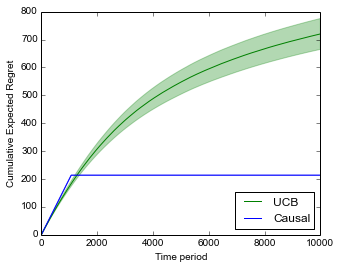
\includegraphics[width=.5\textwidth]{explore_exploit}
\end{figure}

\pagebreak

\section{Generalizing to unbalanced $\boldsymbol{q}$}

\subsection{Option 1: Targeted sampling during exploration phase}

The key fact we were utilizing to draw conclusions about multiple arms during each timestep of the explore phase is that, given our assumed causal structure, $P(Y|do(X_i=j)) = P(Y|X_i=j)$ 

If we do some form of targeted sampling, where we say opt to select each action $I = do(X_a = b)$ some specified number of times $\tau_{ab}$, then we can no longer estimate $P(Y|X_i=j)$ simply by from the proportion of successes given $X_i=j$. 

\eqn {
P(Y|do(X_i=j)) &= P(Y|X_i = j)\\
 &= \sum_{b}P(Y|X_i = j,X_a = b)P(X_a = b|X_i = j) \\
 &= \sum_{b}P(Y|X_i = j,X_a = b)P(X_a = b), \; \forall \, a \in \{1...K\}/i \text{ as } X_a \ci X_i\\
 \label{eqn:marginalizedEstimator}
 &= \sum_{b}P(Y|X_i = j,do(X_a = b))P(X_a = b) 
}

Define $\mu^{ij} = E[Y|X_i=j] = P(Y|X_i=j)$

Let $\hat{\mu}_a^{ij}$ be an estimator for $\mu^{ij}$ based on samples where the intervention was on variable $a$.
\eqn {
\hat{\mu}_a^{ij} &=
\begin{cases}
\label{eqn:marginalizedEstimator2}
\frac{1}{q_i(j)}\left(\frac{m_{a,1}^{ij}}{\tau_{a1}}q_a+\frac{m_{a,0}^{ij}}{\tau_{a0}}(1-q_a)\right) & \text{if } a \neq{i} \\
\frac{m_{i,j}^{ij}}{\tau_{ij}} & \text{if } a=i \\
\end{cases}\\
}

where 

\eqn{
m_{a,b}^{ij} &= \sum_{s \in \{t:I_t=(a,b)\}} Z_{ab,s}^{ij} \text{ and,}\\
Z_{ab,s}^{ij} &= \ind{X_{i,s} = j,Y_s=1} \in \{0,1\}
}

TODO check/show this estimator is unbiased

For each arm, specified by the tuple $i,j$, we now have $K$ estimators $[\hat{\mu}_1^{ij}...\hat{\mu}_K^{ij}]$ which we wish to combine to form a single estimator $\hat{\mu}^{ij}$. We will pool them as a weighted average with weights we can optimize based on the $q's$ so as to minimize the variance of the estimator.

\eqn{
\hat{\mu}^{ij} = \sum_{a=1}^K w_{a} \hat{\mu}_{a}^{ij} \;\;\text{, where } \sum_{a=1}^K w_a = 1
}

Putting everything together,

\eqn{
\hat{\mu}^{ij} = \frac{w_i}{\tau_{ij}}\sum_{s \in \{t: I_t = (i,j)\}} Z_{ij,s}^{ij} + \sum_{a \neq i} \left(\frac{w_a}{q_i(j)}\left[ \frac{q_a}{\tau_{a1}}\sum_{s \in \{t:I_t=(a,1)\}} Z_{a1,s}^{ij}+  \frac{1-q_a}{\tau_{a0}}\sum_{s \in \{t:I_t = (a,0)\}} Z_{a0,s}^{ij} \right] \right)
}

We now need to show $E[\hat{\mu}^{ij}] = \mu^{ij}$ and get a high probability bound for their difference. For the latter, lets try and use McDiarmids Inequality. 

McDiarmid's Inequality states:
If $Z_i \ci Z_j$ and 
\eqn{
|\phi(Z_1...Z_i...Z_N) - \phi(Z_1...Z_i^{'}...Z_N)| < c_i \;\; \forall i
}
\eqn{
\label{eqn:McDiarmid}
& P\left(|\phi(\boldsymbol{Z}) - E[\phi(\boldsymbol{Z})]| \geq \epsilon \right) \leq 2 \exp \left(-\frac{2 \epsilon^2}{\sum_{i}c_i^2} \right)\\
& P\left(|\phi(\boldsymbol{Z}) - E[\phi(\boldsymbol{Z})]| \geq 
\sqrt{\frac{\sum_{i}c_i^2}{2}\log{\frac{2}{\delta}}} 
\right) \leq \delta
}

For our problem, $\hat{\mu}^{ij} = \phi(\boldsymbol{Z}^{ij})$. All the $Z's$ are independent as they correspond indicator functions over the results at different timesteps. 

\eqn{
|\phi(...Z_{ij,s}^{ij}...) - \phi(...Z_{ij,s}^{'ij}...)| & \leq \frac{w_i}{\tau{ij}}\;\;\;\; \leftarrow \tau_{ij} \text{ such $Z$'s}\\
|\phi(...Z_{a1,s}^{ij}...) - \phi(...Z_{a1,s}^{'ij}...)| & \leq \frac{w_a q_a}{q_i(j)\tau_{a1}} \;\;\;\; \leftarrow \tau_{a1} \text{ such $Z$'s for each $a$}\\
|\phi(...Z_{a1,s}^{ij}...) - \phi(...Z_{a1,s}^{'ij}...)| & \leq \frac{w_a (1-q_a)}{q_i(j)\tau_{a0}} \;\;\;\; \leftarrow \tau_{a0} \text{ such $Z$'s for each $a$}
}

\eqn{
\label{eqn:sum_ci}
\sum_l c_l^2 = & \frac{w_i^2}{\tau_{ij}} + \sum_{a \neq i}\frac{w_a^2}{q_i(j)^2}\left(\frac{q_a^2}{\tau_{a1}} +\frac{(1-q_a)^2}{\tau_{a0}}  \right)\\
= & \sum_{a=1}^K w_a^2 f(a) \text{, where} \\
f(a) =& \begin{cases}
\frac{1}{q_i(j)^2}\left(\frac{q_a^2}{\tau_{a1}}+  \frac{(1-q_a)^2}{\tau_{a0}}\right)  & a \neq i\\
\frac{1}{\tau_{ij}} & a = i
\end{cases} 
}

We want to select weights to minimize equation \ref{eqn:sum_ci} so as to achieve as tight a bound as possible in equation \ref{eqn:McDiarmid}.

Applying Legrange Multipliers

\eqn {
w_a & = \frac{1}{f(a)\sum_a \frac{1}{f(a)}} \\
\label{eqn:min_sum_ci}
\sum_i c_i^2 & = \frac{1}{\sum_a \frac{1}{f(a)}}
}

Substitution \ref{eqn:min_sum_ci} back into \ref{eqn:McDiarmid}

\eqn {
& P\left(|\hat{\mu}^{ij} - \mu^{ij}| \geq \epsilon \right) \leq 2 \exp \left(-2 \epsilon^2 \sum_{a=1}^K \eta_a^{ij} \right)\\
& \eta_a^{ij} = \begin{cases}
\frac{\tau_{a1} \tau_{a0} q_i(j)^2}{\tau_{a1}(1-q_a)^2+\tau_{a0}q_a^2} & a \neq i\\
\tau_{ij} & a = i
\end{cases} \\
}

Substituting this into \ref{eqn:probDeltaToLarge}

\eqn{
\label{eqn:targeted_prob_delta_too_big}
P(\Delta_{\hat{i^*}} > D) \leq 2 \sum_{(i,j)} exp\left({-\frac{D^2}{2} \sum_{a=1}^K \eta_a^{ij}}\right)
}

\eqn{
R_2 \leq (T-h)\left(D+2 \sum_{(i,j)} exp\left({-\frac{D^2}{2} \sum_{a=1}^K \eta_a^{ij}}\right) \right)
}

Looking at equation \ref{eqn:targeted_prob_delta_too_big}, let $A = \frac{D^2}{2}$ and

\eqn{
c_a =  \frac{\tau_{a1}\tau_{a0}}{\tau_{a1}(1-q_a)^2+\tau_{a0}q_a^2}
}

\eqn{
f(\boldsymbol{\tau}) := \frac{1}{2}P(\Delta_{\hat{i^*}} > D)  =  \sum_{i=1}^N e^{-A ( \tau_{i1} + q_{i}^2 \sum_{a \neq i} c_a  )}+\sum_{i=1}^N e^{-A ( \tau_{i0} + (1-q_{i})^2 \sum_{a \neq i} c_a)}
}

The goal is to find some assignment $\boldsymbol{\tau}(\boldsymbol{q})$ to minimize this subject to the constraint that $\sum_i \tau_{i1} + \sum_i \tau_{i0} = h$

No luck attempting to do this directly (via Lagrange multipliers ...)

Note, letting $\tau_a = \tau_{a1}+\tau_{a0}$ then $c_a$ is maximized to equal $\tau_a$ if $\tau_{a1} = q_a \tau_a$ 

Consider the case where we have only 2 variables.

\eqn{
f(\boldsymbol{\tau}) = e^{-A(\tau_{11} + q_1^2 c_2)}+
e^{-A(\tau_{21} + q_2^2 c_1)}+
e^{-A(\tau_{10} + (1-q_1)^2 c_2)}+
e^{-A(\tau_{20} + (1-q_2)^2 c_1)}
}

If we consider the extreme case where $q_1=q_2=1$, ie the arms $X_1=0$ and $X_2=0$ never occur naturally. 

\eqn{
f(\boldsymbol{\tau}) = 2 e^{-A(\tau_{11} + \tau_{21})}+
e^{-A(\tau_{10})}+
e^{-A(\tau_{20})}
}

Which is minimized subject to the constraint $\tau_{11}+\tau_{10}+\tau_{21}+\tau_{20}=h$ if we let $\tau_{10}=\tau_{20} = \frac{Ah-log(2)}{3A}$. Note that as $h$ gets large, we play the arms that do not occur naturally roughly $\frac{1}{3}$ of the time as opposed to $\frac{1}{4}$ if we were to play uniformly.  We only learn anything about the arms that do not naturally occur when we play them directly. For the other arms we learn something all the time (provided we have some level of balance in all the other arms...) so it makes sense to play the arms that don't occur naturally a little bit more to keep the overall bounds tight. 

Ok, what happens if we just let $\tau_{ij} = \frac{h}{K}$

\eqn {
c_a = \frac{h}{K}\left(\frac{1}{(1-q_a)^2+q_a^2} \right) \geq \frac{h}{K}
}

\eqn {
f \leq \sum_{i=1}^N \left(e^{-A(\frac{h}{K}+q_i^2\frac{(K-1)}{K}h)}+ e^{-A(\frac{h}{K}+(1-q_i)^2\frac{(K-1)}{K}h)}\right) \\
\leq \sum_{i=1}^N \left(e^{-Ah}+ e^{-A(\frac{h}{K})}\right)
}

Basically worst case, we learn about half the arms fast.

More generally, it would seem by targeted sampling we should be able to learn all the arms with reasonable natural probability fast - and the remaining arms at the rate $h/K$ (or better if we play them more often). 

Approaches to finding some better sampling function.

\begin{enumerate}
\item Find something motivated by the two variable example and show that it performs better than the uniform sampling approach.
\item  Consider some other edge cases 
\end{enumerate} 

Lets consider the case $q_1 = 1, q_2...q_N = \frac{1}{2}$ We will have $\tau_{11},\tau_{10},\tau_{ij} = \tau \; \forall i > 1,j$

\eqn {
c_a = \begin{cases}
\tau_{11} & \text{ if } a=1\\
2 \tau & \text{ otherwise}
\end{cases}
}


\eqn{
f(\boldsymbol{\tau}) & = e^{-A(\tau_{11}+2(N-1)\tau)} + e^{-A\tau_{10}} + 2 (N-1) e^{-A (\tau + \frac{1}{4}(\tau_{11}+2(N-2)\tau))} \\
& = e^{-A(\tau_{11}+2(N-1)\tau)} + e^{-A\tau_{10}} + 2 (N-1) e^{-A (\frac{\tau_{11}}{4} + \frac{N\tau}{2})} \\
& <  e^{-A\tau_{10}} + (2 (N-1)+1) e^{-A (\frac{\tau_{11}}{4} + \frac{N\tau}{2})}\\
& =  e^{-A\tau_{10}} + (2N-1) e^{-A (\frac{\tau_{11}}{4} + \frac{N\tau}{2})}
}

and the constraint is $\tau_{11}+\tau_{10}+2(N-1)\tau = h$

If we maximize $(\frac{\tau_{11}}{4} + \frac{N\tau}{2})$ subject to $\tau_{11}+2(N-1)\tau = (h-\tau_{10})$ we find $\tau = \frac{h-\tau_{10}}{2(N-1)}$ and $\tau_{11} = 0$. Note, as $N$ gets large the sensitivity to the trade off between $\tau$ and $\tau_{11}$ becomes negligible.

\eqn {
\frac{\tau_{11}}{4} + \frac{N\tau}{2} = \begin{cases}
\frac{(h-\tau_{10})N}{4(N-1)} & \text{if } \tau_{11}=0 \\
\frac{(h-\tau_{10})N}{4(N-1)} - \frac{1}{4(N-1)} &\text{if } \tau_{11}=(h-\tau_{10})
\end{cases}
}

\eqn {
f(\boldsymbol{\tau}) & <e^{-A\tau_{10}} + (2N-1) e^{-A (\frac{1}{4}(h-\tau_{10}))}
}

Which is minimized if 
\eqn {
\tau_{10} = \frac{h}{5} - \frac{4}{5A}log(\frac{2N-1}{4})
}

Ok - lets look at the reverse case, where $q_1=\frac{1}{2}, q_2...q_N = 1$

\eqn{
\sum_a c_a = \begin{cases}
(N-1)\tau_{11} & \text{ if } a = 1 \\
2\tau+(N-2)\tau_{11} &\text{ otherwise }
\end{cases}
}

The constraint is 
\eqn {
2\tau+(N-1)\tau_{11} + (N-1)\tau_{10} = h
}

\eqn{
f(\boldsymbol{\tau}) = 2e^{-A(\tau+\frac{1}{4}(N-1)\tau_{11})} + (N-1)e^{-A(2\tau+(N-1)\tau_{11})}+(N-1)e^{-A\tau_{10}}
}

Holding $\tau_{10}$ constant, the 2nd and 3rd terms are constant. The first is maximized by letting $\tau_{11} = 0, \tau = \frac{h - (N-1)\tau_{10}}{2}$

\eqn{
f(\boldsymbol{\tau}) & = 2e^{-A\tau} + (N-1)e^{-2A\tau}+(N-1)e^{-A\frac{h - 2\tau}{N-1}} \leftarrow \text{ can't minimize analytically} \\
\label{eqn:case1balancedapprox}
& \leq (N+1)e^{-A\tau} +(N-1)e^{-A\frac{h - 2\tau}{N-1}}
}

which is minimized if 

\eqn {
\tau & = \frac{1}{N+2}\left( h - N + \frac{N}{A} \log(\frac{N(N+1)}{2(N-1)})\right) \\
\label{eqn:case1balancedapproxsolution}
& \sim \frac{1}{N+2}\left( h - N + \frac{N}{A} \log(\frac{N}{2})\right)
}

Equation \ref{eqn:case1balancedapproxsolution} is also the solution that leads to the exponentiated terms in equation \ref{eqn:case1balancedapprox} being equal - which is should intuitively be optimal since the coefficients in front of them are very similar.

Yet another case study - if $q_1...q_N = 1$ So none of the arms $X_i = 0$ occur naturally.

\eqn{
&c_a  = \tau_1 \; \forall a\\
&\sum_{i \neq a}c_a  = (N-1)\tau_1 \; \forall a\\
& N(\tau_0+\tau_1) = h\\
& f(\boldsymbol{\tau}) = N e^{-A N\tau_1} + N e^{-A\tau_0}
}

minimized if 
\eqn{
\tau_0 = \frac{h}{N+1}-\frac{log(N)}{A(N+1)}
}

Note as $N$ get large - this equates to $\tau_0 \sim \frac{h}{N}$ ie almost all the actions are allocated to the arms that do not occur naturally. 


Another case study $q_1...q_{N_1} = 1,q_{N_1+1}...q_N = \frac{1}{2}$ (should encompass all previous examples ...)

\eqn{
&c_a  = \begin{cases}
\tau_{11} &\text{ if } a \leq N_1
 \\
2\tau & \text{otherwise}
\end{cases}\\
&\sum_{i \neq a}c_a  = \begin{cases}
(N_1-1)\tau_{11} + 2 N_2 \tau & \text{ if } a \leq N \\
N_1\tau_{11} + 2(N_2-1)\tau & \text{ otherwise }
\end{cases}\\
&N_1\tau_{10}+N_1\tau_{11}+2N_2\tau = h\\
&f(\boldsymbol{\tau}) =  N_1 e^{-A\tau_{10}}+ N_1 e^{-A(N_1\tau_{11}+2N_2\tau)} + 2N_2 e^{-A(\frac{N_1}{4}\tau_{11}+\frac{N_2+1}{2}\tau)}
}

The 2nd and 3rd terms are minimized by letting $\tau_{11} = 0$ (although the result is only weakly dependnent on the trade off between $\tau_{11}$ and $\tau$ provided $N_2 >> 2$).

\eqn{
f(\boldsymbol{\tau}) &=  N_1 e^{-A\tau_{10}}+ N_1 e^{-A2N_2\tau} + 2N_2 e^{-A\frac{N_2+1}{2}\tau}\\
& \leq N_1 e^{-A\tau_{10}} + (2N_2 + N_1)e^{-A\frac{N_2+1}{2}\tau}\\
& = N_1 e^{-A\tau_{10}} + (2N_2 + N_1)e^{-A(\frac{(N_2+1)(h-N_1\tau_{10})}{4N_2})} 
} 


\eqn{
\tau_{10} = \left(\frac{N_2+1}{(N_2+1)N_1+4N_2}\right)h-\frac{4N_2\log(\frac{(N_2+1)(2N_2+N_2)}{4N_2})}{A((N_2+1)N_1+4N_2))}
}

It seems like this function can be optimized in a greedy way. That is, start with $\boldsymbol{\tau} = \boldsymbol{0}$, and in each timestep select the $\tau_{ij}$ that leads to the greatest reduction in the error bound. This appears to yield broadly consistent results to the analytic solution.

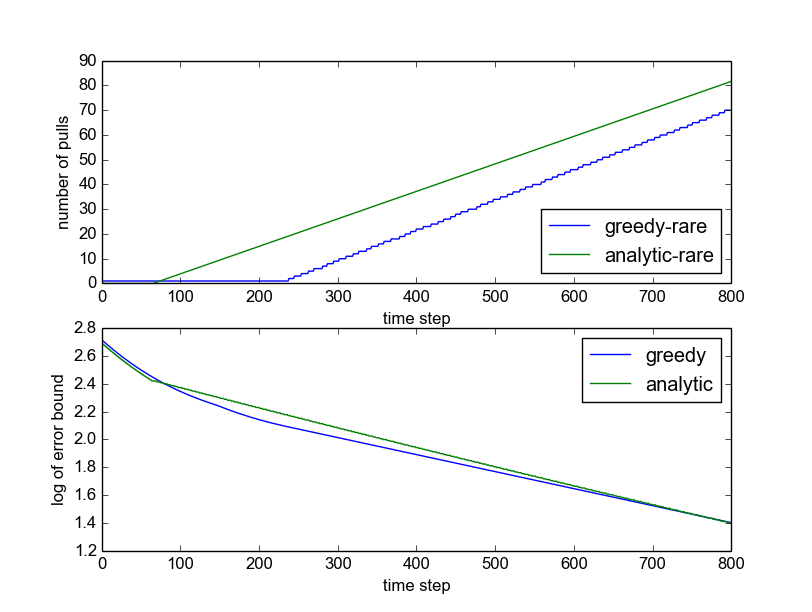
\includegraphics[width=.5\textwidth]{greedy_minimization_close}
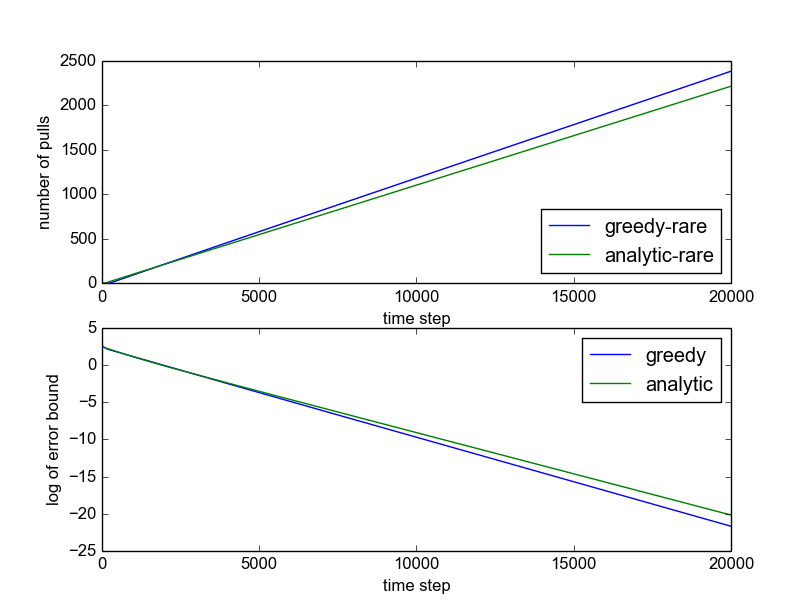
\includegraphics[width=.5\textwidth]{greedy_minimization}


Ok - so when we have many unbalanced variables, we assign almost all actions to the arms corresponding to the rare side. However, this will still be $< h/N$ which is only a factor of $2$ better than uniform assignment. Doing something smarter than uniform assignment will make more difference where we have a only a few unbalanced variables. In this case - smart assignment will lead to bounds almost as tight as the perfectly balanced case. Uniform assignment may yield solutions that are almost as bad as the worst case. (still better than without using the structure at all)

I still need to cover more fractional $q$'s... 



What about if I repeated one of the above analysis but let the unbalanced q = .75?

What can I say overall about worst/best cases/any symmetries in the problem??? Do these solutions lead to the terms in the exponentials being similar?

Goal is to choose something that will give us a simple bound and will be ok for the worst case. Its still not entirely clear to me what the worst case will be - after all it depends on the way you assign to $\tau$.

What happens if we assume $\sum_{a\neq i} c_a$ is constant ... this is reasonable if $N$ is large 

When you look at each term in $c_a$, its maximized if we play the arms according to their natural probabilities. If the arm is balanced, this will also minimize the sum of the two terms for doing $x_i = 0$ and $x_i = 1$. If the arm is unbalanced, then we have to trade of balancing this sum versus contributing to the sum of $c_a$. Consider just how bad the sum of $c_a$ can be even if we focus entirely on balancing the two terms ... maybe its already enough.

Fundamentally the relationship between arms is complex. Its not that we get any direct link from one arm to another - rather pairs of actions tell us something about other arms.   


\pagebreak


\subsection{Option 2: Some measure of information gain}

\subsection{Option 3: Three stage algorithm}
\begin{enumerate}
\item Observe randomly
\item Play low probability arms
\item Pick best and exploit
\end{enumerate}

\pagebreak

\end{document}


